\documentclass[12pt]{article}
\usepackage[margin=1.5cm]{geometry}
\usepackage{xcolor} % For custom colors
\usepackage{listings}
\usepackage{graphicx}
\graphicspath{ {./images/Lab8} }

% Define SQL style
\lstdefinelanguage{SQL}{
  morekeywords={
    ALTER, ADD, DROP, SELECT, FROM, WHERE, AND, OR, INSERT, INTO, VALUES, UPDATE, SET, DELETE,
    VARCHAR, INT, DATE, FLOAT, BOOLEAN,
    CREATE, TABLE, PRIMARY, KEY, FOREIGN, NOT, NULL, REFERENCES, INNER, OUTER, NATURAL, JOIN, CONSTRAINT,
    LEFT, RIGHT, FULL, ON, AS, USING, DISTINCT, GROUP, BY, ORDER, HAVING, LIMIT, UNIQUE, CASCADE, DEFAULT,
    RENAME, DESCRIBE, TO, IN, IF, CASE, WHEN, THEN, ELSE, END, TIMESTAMPDIFF, CURRENT_DATE, ROUND, CONCAT,
    UNION, WITH, SOME, ALL, EXISTS, ANY, SUM, AVG, COUNT, MIN, MAX, DETERMINISTIC, BEGIN, END, BETWEEN, DECLARE,
    DELIMITER, PROCEDURE, FUNCTION, TRIGGER, BEFORE, AFTER, INOUT, OUT, CALL, FOR, EACH, ROW, RETURN, RETURNS
  },
  sensitive=false,
  morecomment=[l]{--}, % SQL single-line comments
  morecomment=[s]{/*}{*/}, % SQL multi-line comments
  morestring=[b]', % Strings in single quotes
}
\definecolor{darkgreen}{rgb}{0,0.4,0}
\lstset{language=SQL,
    numbers=left,
    basicstyle=\ttfamily,
    showstringspaces=false,
    keywordstyle=\color{blue}\bfseries,
    commentstyle=\color{orange}\itshape,
    stringstyle=\color{darkgreen},
    frame=single,
    breaklines=true
}
    
\begin{document}
\title{CSCD 327 Lab 8}
\author{Dustin Randall}
\maketitle

\section{Find Appointments By Doctor}
\begin{lstlisting}
DELIMITER $
CREATE FUNCTION apptCount(docId INT)
RETURNS INT
DETERMINISTIC
BEGIN
  DECLARE r INT;
  SELECT COUNT(*) INTO r
  FROM appointments
  WHERE doctorID = docId;
  RETURN r;
END $
DELIMITER ;
\end{lstlisting}
\begin{lstlisting}
SELECT doctorID, apptCount(doctorID) as AptCount
FROM doctors
WHERE doctorID IN(12, 14, 18);
\end{lstlisting}

\begin{figure}[ht]
     \centering
     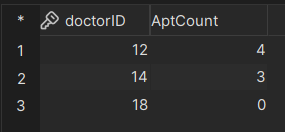
\includegraphics{AptCountByDoc.png}
     \caption{Finding appointment counts by doctor}
 \end{figure}
\pagebreak

\section{Find Recent Appointment}
\begin{lstlisting}
DELIMITER $
CREATE FUNCTION recentApt(patID INT, docID INT)
RETURNS DATE
DETERMINISTIC
BEGIN
  DECLARE r DATE;
  SELECT MAX(appointment_date) INTO r
  FROM appointments
  WHERE patientID = patID AND doctorID = docID;
  RETURN r;
END $
DELIMITER ;
\end{lstlisting}
\begin{lstlisting}
SELECT recentApt(1, 11) AS apt;
\end{lstlisting}

\begin{figure}[ht]
     \centering
     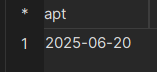
\includegraphics{RecentApt.png}
     \caption{Finding recent appointment date}
 \end{figure}
\pagebreak

\section{Find Appointments By Names}
\begin{lstlisting}
DELIMITER $
CREATE FUNCTION namedAptCount(patFirst VARCHAR(50), patLast VARCHAR(50), docFirst VARCHAR(50), docLast VARCHAR(50))
RETURNS INT
DETERMINISTIC
BEGIN
  DECLARE r INT;
  SELECT COUNT(*) INTO r
  FROM appointments
  WHERE doctorID = (
    SELECT doctorID
    FROM doctors
    WHERE first_name = docFirst AND last_name = docLast
  ) AND patientID = (
    SELECT patientID
    FROM patients
    WHERE first_name = patFirst AND last_name = patLast
  );
  RETURN r;
END $
DELIMITER ;
\end{lstlisting}
\begin{lstlisting}
SELECT namedAptCount('Jane', 'Smith', 'James', 'Wilson') AS aptCount
\end{lstlisting}

\begin{figure}[ht]
     \centering
     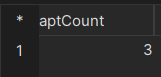
\includegraphics{NamedAptCount.png}
     \caption{Finding appointment count by names}
 \end{figure}
\pagebreak

\section{Find Average Health}
\begin{lstlisting}
DELIMITER $
CREATE PROCEDURE avgHealth(patFirst VARCHAR(50), patLast VARCHAR(50))
DETERMINISTIC
BEGIN
SELECT ROUND(AVG(heart_rate_bpm), 2) AS avgBpm,
  ROUND(AVG(cholesterol_mg_dl), 2) AS avgCol,
  ROUND(AVG(bmi), 2) AS avgBmi
FROM medicalRecords
WHERE patientID = (
  SELECT patientID FROM patients
  WHERE first_name = patFirst AND last_name = patLast
  );
END $
DELIMITER ;
\end{lstlisting}
\begin{lstlisting}
CALL avgHealth('John', 'Doe');
\end{lstlisting}

\begin{figure}[ht]
     \centering
     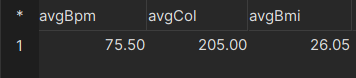
\includegraphics{AvgHealth.png}
     \caption{Finding average health metrics for a patient}
 \end{figure}
\pagebreak

\section{Find Apts And Records By Dates}
\begin{lstlisting}
DELIMITER $
CREATE PROCEDURE aptsAndRecordsByDates(startDate DATE, endDate DATE, OUT aptCount INT, OUT recordCount INT)
DETERMINISTIC
BEGIN
SELECT COUNT(*) INTO aptCount
FROM appointments
WHERE appointment_date BETWEEN startDate AND endDate;
SELECT COUNT(*) INTO recordCount
FROM medicalRecords
WHERE visit_date BETWEEN startDate AND endDate;
END $
DELIMITER ;
\end{lstlisting}
\begin{lstlisting}
SET @AptCount = 0;
SET @RecordCount = 0;
CALL aptsAndRecordsByDates('2025-07-01', '2025-10-31', @AptCount, @RecordCount);
SELECT @AptCount AS aptCount, @RecordCount AS recordCount;
\end{lstlisting}

\begin{figure}[ht]
     \centering
     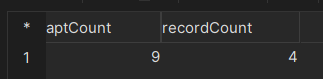
\includegraphics{AptAndRecords.png}
     \caption{Finding appointment and record counts by date range}
 \end{figure}
\pagebreak

\section{Find Patient Doctor Specialties Count}
\begin{lstlisting}
DELIMITER $
CREATE PROCEDURE patientSpecialties(INOUT idAndResult INT)
DETERMINISTIC
BEGIN
SELECT COUNT(DISTINCT specialty) INTO idAndResult
FROM doctors
WHERE doctorID IN (
  SELECT DISTINCT doctorID
  FROM appointments
  WHERE patientID = idAndResult
);
END $
DELIMITER ;
\end{lstlisting}
\begin{lstlisting}
SET @idAndResult = 1;
CALL patientSpecialties(@idAndResult);
SELECT @idAndResult AS result;
\end{lstlisting}

\begin{figure}[ht]
     \centering
     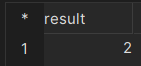
\includegraphics{PatientSpecialties.png}
     \caption{Finding patient doctor specialties count}
 \end{figure}
\pagebreak

\section{Set default insurance values}
\begin{lstlisting}
DELIMITER $
CREATE TRIGGER defaultInsurance
BEFORE INSERT ON insurance
FOR EACH ROW
BEGIN
  SET new.plan_type = 'Platinum';
  SET new.coverage_percent = 96;
  SET new.annual_limit = 35000;
  SET new.deductible = 200;
END $
DELIMITER ;
\end{lstlisting}
\begin{lstlisting}
INSERT INTO insurance(insuranceID, provider_name) VALUES(201, 'Dewie Cheatum and Howe');
SELECT * FROM insurance WHERE insuranceID = 201;
\end{lstlisting}

\begin{figure}[ht]
     \centering
     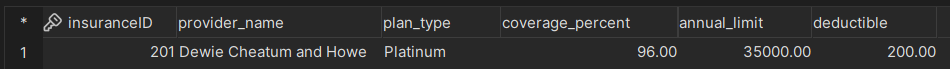
\includegraphics{NewInsurance.png}
     \caption{Setting default insurance values}

 \end{figure}
\pagebreak

\section{Track Prior Providers}
\begin{lstlisting}
CREATE TABLE pastProviders(name VARCHAR(100), plan_type VARCHAR(50));
\end{lstlisting}
\begin{lstlisting}
DELIMITER $
CREATE TRIGGER pastProviderAudit
AFTER DELETE ON insurance
FOR EACH ROW
BEGIN
  INSERT INTO pastProviders VALUES(old.provider_name, old.plan_type);
END $
DELIMITER ;
\end{lstlisting}
\begin{lstlisting}
DELETE FROM insurance WHERE insuranceID = 201;
SELECT * FROM pastProviders;
\end{lstlisting}

\begin{figure}[ht]
     \centering
     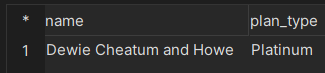
\includegraphics{AuditProviders.png}
     \caption{Tracking prior insurance providers}

 \end{figure}

\end{document}